\section{Evaluation}\seclabel{Evaluation}

\subsection{Latency and Throughput}
{\begin{figure*}[ht]
  \centering
  \begin{subfigure}[c]{0.36\textwidth}
    \centering
    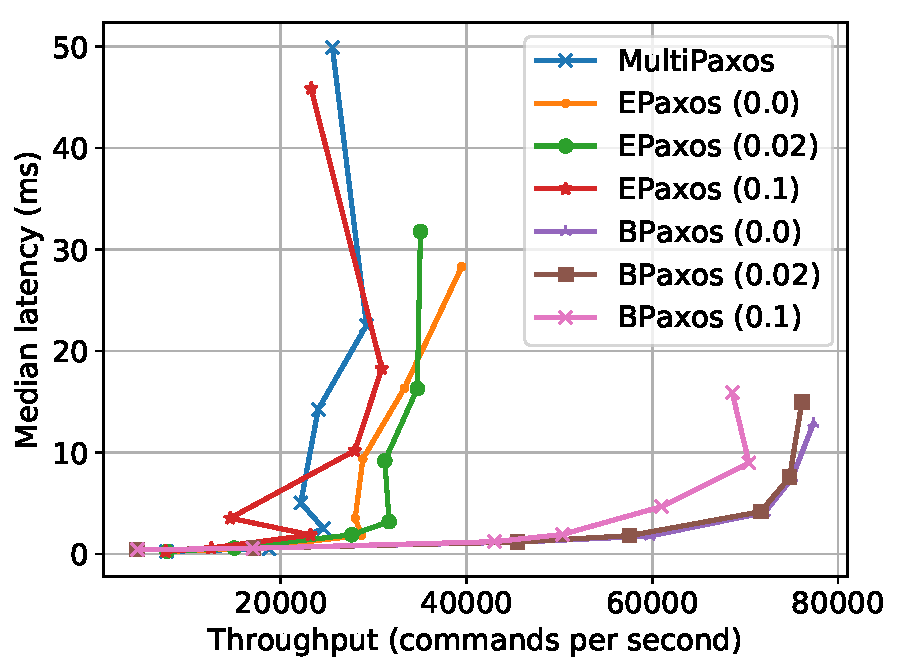
\includegraphics[width=\textwidth]{assets/nsdi_fig1_lt_f1.pdf}
    \caption{
      Latency-throughput curves for Multipaxos, EPaxos, and BPaxos. EPaxos and
      BPaxos are run with 0\%, 2\% and 10\% conflict rates. Here, $f = 1$.
    }\figlabel{EvalLtF1}
  \end{subfigure}
  \begin{subfigure}[c]{0.36\textwidth}
    \centering
    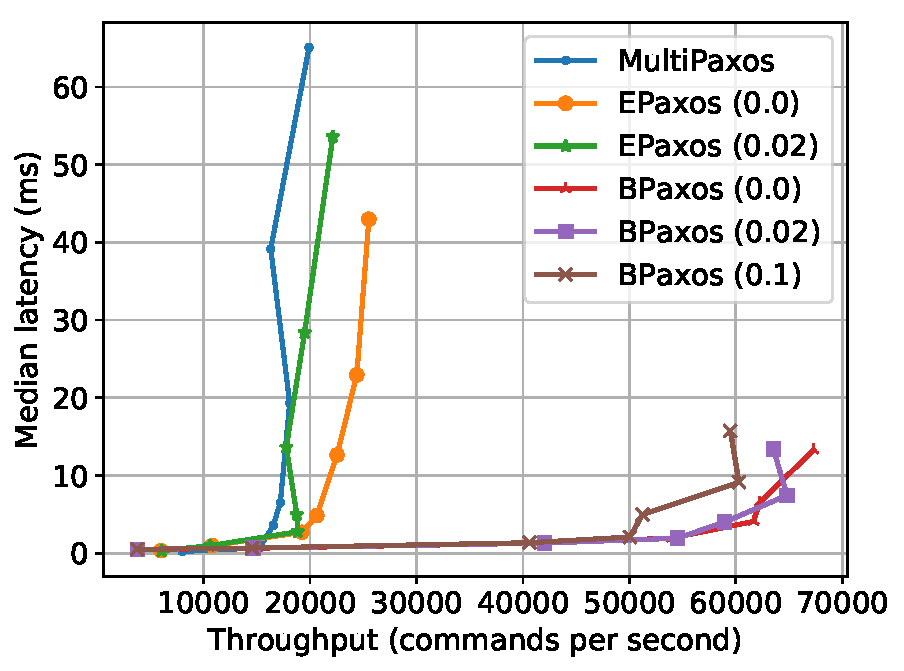
\includegraphics[width=\textwidth]{assets/nsdi_fig1_lt_f2.pdf}
    \caption{The same as \figref{EvalLtF1} but with $f=2$.}%
    \figlabel{EvalLtF2}
  \end{subfigure}
  \begin{subfigure}[c]{0.23\textwidth}
    \centering
    \small
    \begin{tabular}{lccc}
      \toprule
      \multicolumn{1}{c}{Protocol} &
      \multicolumn{3}{c}{Number of clients} \\
      %
                    & 1    & 10   & 50 \\\midrule
      Multipaxos    & 0.24 & 0.52 & 2.49 \\
      EPaxos (0.0)  & 0.25 & 0.56 & 1.83 \\
      EPaxos (0.02) & 0.25 & 0.57 & 1.89 \\
      EPaxos (0.1)  & 0.25 & 0.58 & 1.87 \\
      BPaxos (0.0)  & 0.41 & 0.56 & 1.16 \\
      BPaxos (0.02) & 0.41 & 0.56 & 1.17 \\
      BPaxos (0.1)  & 0.41 & 0.55 & 1.21 \\
      \bottomrule
    \end{tabular}
    \caption{%
      Median latency values (ms) from \figref{EvalLtF1}.
    }\figlabel{EvalLtTable}
  \end{subfigure}
  \caption{%
    Latency and throughput of Multipaxos, EPaxos, and BPaxos for varying number
    of clients, conflict rates, and values of $f$. Data is shown for $1$, $10$,
    $50$, $100$, $300$, $600$, and $1200$ clients.
  }\figlabel{EvalLt}
\end{figure*}
}

\paragraph{Experiment Description.}
We implemented MultiPaxos, EPaxos\footnote{Note that we implement \emph{Basic}
EPaxos, the algorithm outlined in~\cite{moraru2013proof}. Basic EPaxos has
larger quorums and simpler recovery compared to the complete EPaxos protocol
which is described in~\cite{moraru2013there}.}, and BPaxos in Scala. Here, we
measure the throughput and latency of the three protocols with respect to three
parameters: the number of clients, the conflict rate, and the parameter $f$.

\begin{itemize}
  \item \textbf{Clients.}
    Clients propose commands serially. That is, after a client proposes a
    command, it waits to receive a response before proposing another command.
    We also run multiple clients in the same process, so deployments with a
    large number of clients (e.g., $1,200$ clients) may use only a few client
    processes. We run $1$, $10$, $50$, $100$, $300$, $600$, and $1200$ clients.

  \item \textbf{Conflict rate.}
    The protocols replicate a key-value state machine. Commands are single key gets
    or single key sets. With a conflict rate of $r$, $r$ of the commands are sets
    to a single key, while $(1 - r)$ of the commands are gets to other keys. Keys
    and values are both eight bytes. If commands are large, the data path and
    control path can be split, as in~\cite{biely2012s}. We run with $r=0$,
    $r=0.02$, and $r=0.1$. As described in~\cite{moraru2013there}, workloads in
    practice often have very low conflict rates.

  \item \textbf{$f$.}
    Recall that a protocol with parameter $f$ must tolerate at most $f$ failures.
    We run with $f=1$ and $f=2$.
\end{itemize}

We deploy the three protocols on m5.4xlarge EC2 instances within a single
availability zone. MultiPaxos deploys $f+1$ proposers and $2f+1$ acceptors.
EPaxos deploys $2f+1$ replicas. BPaxos deploys $2f+1$ dependency service nodes,
$2f+1$ acceptors, $f+1$ replicas, $5$ leaders and proposers when $f=1$, and
$10$ leaders and proposers when $f=2$. Every logical node is deployed on its
own physical machine, except that every BPaxos leader is co-located with a
BPaxos proposer. The protocols do not perform batching, except that EPaxos and
BPaxos graphs are executed only every 100 commands. This helps amortize the
cost of topological sorting. All three protocols implement thriftiness, a
standard optimization~\cite{moraru2013there}.

% no batching, execpt for graph execution
% thriftiness enabled
% num leaders for experiments
% m5.4xlarge machines in a single availability zone
% key value store with small keys and values, big keys do s-paxos
% clients not all different procs
% explain conflict rate (cite EPaxos saying conflict rates low)
% machine placement
% mention basic epaxos

\paragraph{Results.}
The benchmark results are shown in \figref{EvalLt}. In \figref{EvalLtF1} with
$f=1$, we see that MultiPaxos achieves a peak throughput of roughly 25,000 to
30,000 commands per second. BPaxos achieves a peak throughput of 30,000 to
40,000 depending on the conflict rate. BPaxos achieves 70,000 to 75,000
commands per second, nearly double that of EPaxos. Both EPaxos' and BPaxos'
throughput decrease with higher conflict rate. Higher conflict rates lead to
graphs with more edges, and topological sorting the graphs runs linear in the
number of edges.

Note that the EPaxos implementation in~\cite{moraru2013there} achieves a peak
throughput of 45,000 to 50,000, slightly higher than our implementation. We
believe the discrepancy is due to implementation language (Go vs Scala) and
various optimizations performed in~\cite{moraru2013there} that we have not
implemented (e.g., a custom marshaling and RPC compiler~\cite{epaxos2019blog}).
We believe that if we apply the same optimizations to our implementations, all
three protocols' throughput would increase similarly.

% for f = 1,
% bpaxos peaks out at 75k throughput at low conflict
% at higher conflict, decreases to 70k, more conflict, more cyclces, longer execution
% epaxos 35k-40k low conflict
% epaxos 30k high conflict
% epaxos multipaxos 25-30k

In \figref{EvalLtF2}, with $f=2$, MultiPaxos' peak throughput has decreased to
20,000, EPaxos' peak throughput has decreased to 25,000, and BPaxos' peak
throughput has decreased to 65,000. As $f$ increases, the MultiPaxos leader has
to contact more nodes, so the drop in throughput is expected. With $f=2$,
EPaxos and BPaxos both have more leaders. More leaders increases the likelihood
of cycles, which slow the protocol down slightly. Moreover, when performing
dependency compaction as described in \secref{PracticalConsiderations}, the
number of dependencies scales with the number of leaders. BPaxos's peak
throughput is still roughly double that of EPaxos.

% nearly doubled the throughput
% f=2, similar story higher f, lowers throughput for other protocols
% for us it does a little, but not as much, this is expected for larger f
% more leaders means more deps

After sending a command, a BPaxos client must wait eight network delays to
receive a response. MultiPaxos and EPaxos require only four. Thus, under low
load, MultiPaxos and EPaxos have lower latency than BPaxos. In
\figref{EvalLtTable}, we see that with a single client, MultiPaxos and EPaxos
have a latency of roughly 0.25 ms, whereas BPaxos has a latency of 0.41. Under
high load though, BPaxos achieves lower latency. With 10 clients, the latency
of the three protocols is roughly even, and with 50 clients, BPaxos's latency
has already dropped below that of the other two protocols. In \figref{EvalLtF1}
and \figref{EvalLtF2}, we see that under higher loads of 600 and 1200 clients,
BPaxos's latency can be two to six times lower than the other two protocols.
Note however that these results are specific to our deployment within a single
data center. With a geo-replicated deployment, MultiPaxos and EPaxos would both
outperform BPaxos. In this scenario, minimizing network delays is paramount.

% throughput higher but latency isn't
% look at the latency in fig c
% multipaxos and epaos roughly half the latency, makes sense cause half the network delays
% but at higher load, and with fast networks, latency starts to become dictated by throughput and bpaxos can achieve lower latency and the same throughputs, e.g. 10 clients all same, 50 clients better. in wan, we would see double always pretty much

\subsection{Ablation Study}
{\begin{figure*}[ht]
  \centering
  \begin{subfigure}[b]{0.3\textwidth}
    \centering
    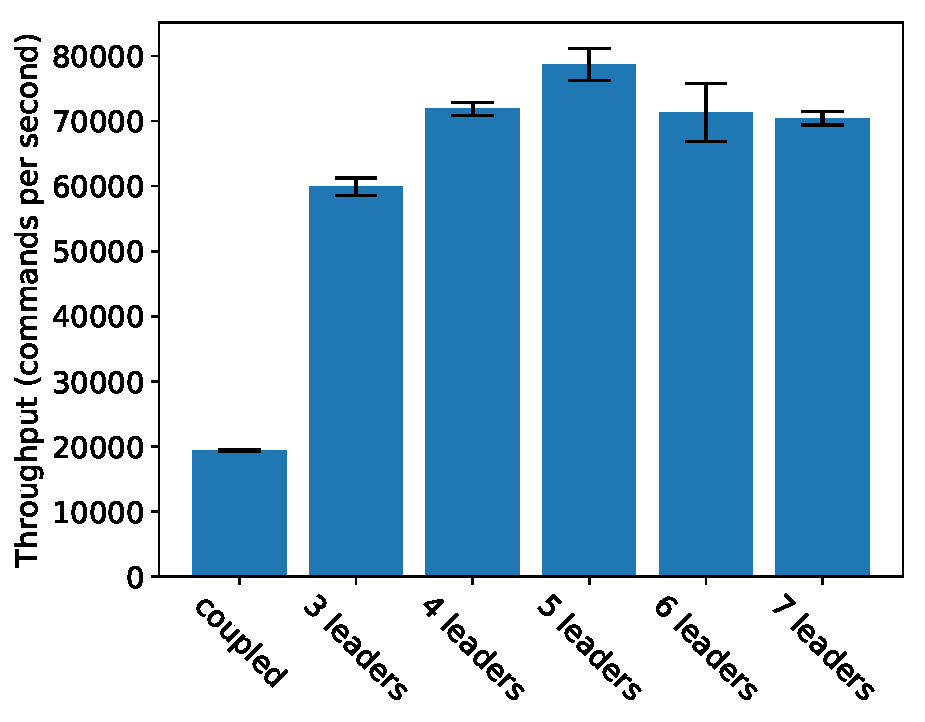
\includegraphics[width=\textwidth]{assets/nsdi_fig2_ablation_high_load_throughput.pdf}
    \caption{Throughput with 600 clients.}%
    \figlabel{EvalAblationHighLoadThroughput}
  \end{subfigure}\hspace{0.03\textwidth}
  \begin{subfigure}[b]{0.3\textwidth}
    \centering
    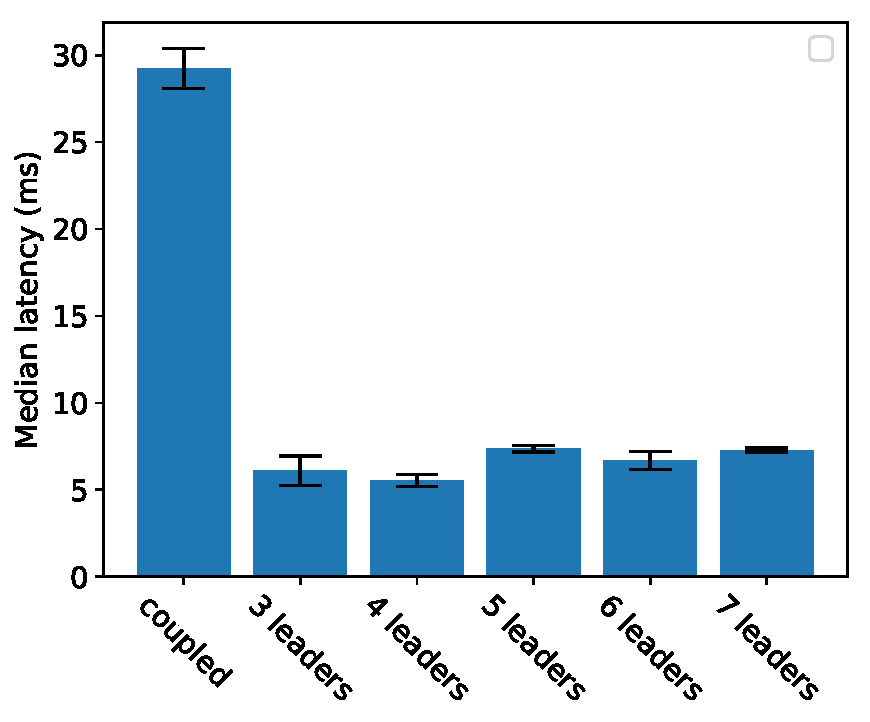
\includegraphics[width=\textwidth]{assets/nsdi_fig2_ablation_high_load_latency.pdf}
    \caption{Median latency (ms) with 600 clients.}%
    \figlabel{EvalAblationHighLoadLatency}
  \end{subfigure}\hspace{0.03\textwidth}
  \begin{subfigure}[b]{0.3\textwidth}
    \centering
    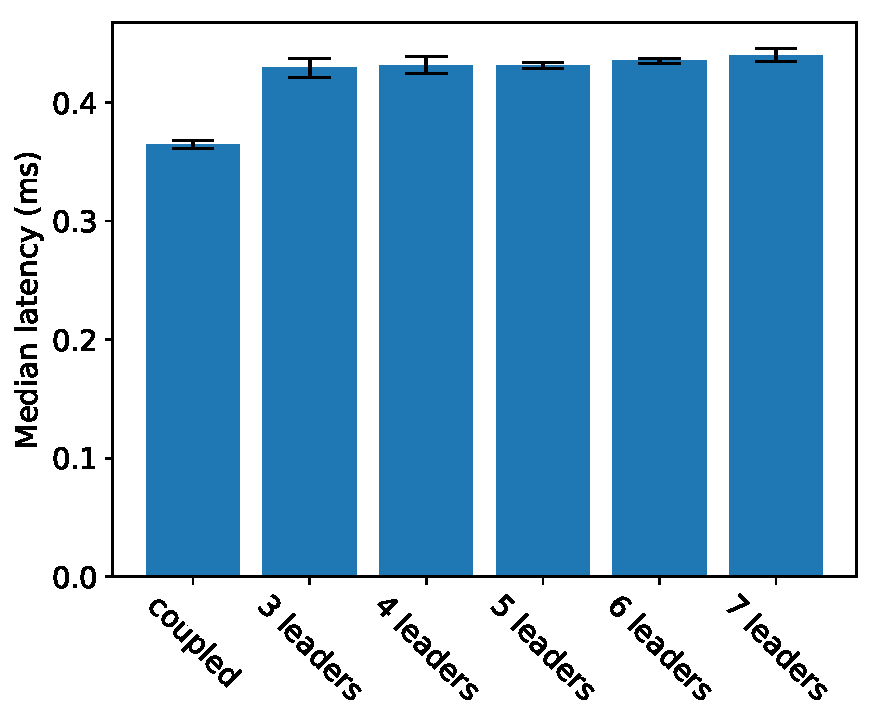
\includegraphics[width=\textwidth]{assets/nsdi_fig2_ablation_low_load_latency.pdf}
    \caption{Median latency (ms) with one client.}%
    \figlabel{EvalAblationLowLoadLatency}
  \end{subfigure}
  \caption{%
    An ablation study showing the effect of disaggregation and scaling on
    throughput and latency with 600 clients and one client. Throughput for one
    client is not shown because it is simply the inverse of latency.
  }\figlabel{EvalAblation}
\end{figure*}
}

\paragraph{Experiment Description.}
The previous experiment showed that BPaxos can achieve roughly double the
throughput of EPaxos. Now, we analyze how BPaxos achieves these speedups. In
particular, we perform an ablation study to measure how BPaxos' disaggregation
and scaling affect its throughput. We repeat the experiment from above with
$f=1$, with $r=0$, and with $1$ and $600$ clients. We vary the number of
leaders from $3$ to $7$. Moreover, we also consider a ``coupled BPaxos''
deployment with three machines where each machine runs a single process that
acts as a leader, a dependency service node, a proposer, an acceptor, and a
replica. This artificially coupled BPaxos is similar to EPaxos in which every
replica plays many roles.

% same setup as above
% run all components in one proc
% scale number of leaders
% see effects of decoupling and scaling
% high and low load

\paragraph{Results.}
The results of the experiment are shown in \figref{EvalAblation}. In
\figref{EvalAblationHighLoadThroughput}, we see the throughput of the coupled
BPaxos deployment is only 20,000 under high load. This is lower than both
MultiPaxos and EPaxos. When we decouple the protocol and run with three
leaders, the throughput increases threefold to 60,000. Disaggregating the nodes
introduces pipeline parallelism and reduces the load on the bottleneck
component. As we increase to five leaders, the throughput increases to a peak
of 75,000. At this point, the leaders are not the bottleneck and adding more
leaders only serves to slow down the protocol (for reasons similar to why the
$f=2$ deployment of BPaxos is slightly slower than the $f=1$ deployment).

In \figref{EvalAblationHighLoadLatency}, we see that the coupled protocol has
roughly six times the latency compared to the decoupled protocol under high
load. Moreover, the number of leaders doesn't have much of an impact on the
latency. In \figref{EvalAblationLowLoadLatency}, we see that the coupled
protocol has lower latency compared to the decoupled protocol under low load,
as fewer messages have to traverse the network. These results are consistent
with the previous benchmarks. Coupled protocols can achieve lower latency under
high load but decoupled protocols achieve higher throughput and lower latency
under high load.

In summary, both disaggregation and scaling contribute significantly to BPaxos'
increased throughput and lower latency under high load, and they also explain
why BPaxos has higher latency under low load.

% under high load, 600 clients, coupled perofrms worse than multipaxos and epaxos
% this is expected, bpaxos now has alot of orles
% when we doucple, we see triplign in throughput, already beating state of the art
% we scale up to 5 leaders to get an aditional 125\% throughput boost. once the leaders are not bottleneck, adding more doesnt help, it can acutallu hurt because more deps
%
% latency is helped by decoupling but leaders doest affect latency much
% at low load, the latency of coupled is slightly lower, fewer messages have to be sent across the network, this latency speedup would be even higher if we performened more aggresive forms of coupling
%
\subsection{Batching}
BPaxos achieves high throughput by decoupling nodes and scaling bottleneck
components. We can increase the throughput even further (at the cost of
latency) by batching. That is, BPaxos leaders can collect batches of commands
from clients and place all of them within a single vertex. Batching improves
the throughput of all replication protocols~\cite{santos2012tuning,
santos2013optimizing, moraru2013proof}, however BPaxos' modular design enables
the protocol to take advantage of batching particularly well.

First, the overheads of receiving client messages and forming batches falls
onto the leaders. Because we can scale the leaders, these overheads can be
amortized until they are no longer a bottleneck. Moreover, proposers and
replicas both run linear with the number of batches, not the number of
commands. Thus, increasing the batch size also amortizes their overheads.
Finally, as batch sizes grow, the number of vertices and edges in the graphs
shrink. Replicas can topologically sort the smaller graphs faster.

We repeated the benchmarks from above with $f=1$ and $r=0$ with a batch size of
$1,000$ and achieved a peak throughput of roughly $500,000$ commands per second
with a median latency of roughly 200 ms.

\TODO[mwhittaker]{Get better batching numbers.}
